\subsection{Current Solution}
\label{description:solution}

Currently, there exists the functionality to create bullet lists and different Tomboy notes with links in between them.
There existed an older project (also realised as an Addin) for task management, which however was removed later because it did not meet the design constraints. It was a totally separate task management UI in Tomboy that was not integrated
into the existing note structure at all. Later, a new project (also in terms of a Addin) was initiated, but never finished and still contains bugs.
Our goal is now to finish such a project up to a stable solution such that it could be included into the official Tomboy project.

\subsection{Product Perspective}
\label{description:perspective}
\textit{
Describe relation with other products if any. Examples:
System interfaces
User interfaces
Hardware interfaces
Software interfaces
Communication interfaces
Memory
Operations
Site adaptation requirements}

The project TaskList will be part of the Tomboy project. There will be three main interfaces. The first one is the obvious user interface as used by the user through Tomboy. Then, representing data will be done via Tomboy note files. Saving and retrieving data will be using XML files. 

\begin{figure}[h]
 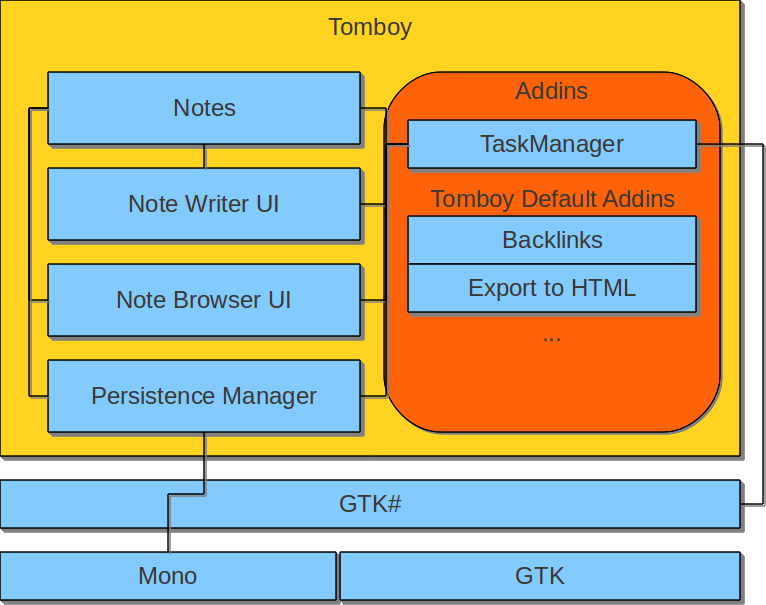
\includegraphics[width=\textwidth]{graphics/product_perspective_diagram.png}
 \caption{TaskList Product Perspective}
 \label{gui}
\end{figure}


\subsection{Product Functions}
\label{description:functions}
\textit{
Write a summary of the major functions that the software will perform. The functions should be organized in a way that makes the list of functions understandable to the customer or to anyone else reading the document for the first time. Textual or graphical methods can be used to show the different functions and their relationships.
}
	\subsubsection*{Supported Functions}
	\label{description:functions:supported}
	\begin{itemize}
		\item Provides a task management Addin for Tomboy
                \item Supports multiple tasks and tasklists as well as subtasks
                \item Allows to create dependencies between tasks
                \item Allows to manage task lists and tasks
                \item 
	\end{itemize}

	\subsubsection*{Unsupported Functions}
	\label{description:functions:unsupported}
	\begin{itemize}
		\item Does not have additional GUI elements or external tools within or outside of Tomboy. (SEE ?)
		\item Does not support synchronisation with external tools or clients except for manual export.
	\end{itemize}
	

\subsection{User Characteristics}
\label{description:usercharacteristics}
\begin{itemize}
\item Casual user
The casual user will create simple task lists. He knows the basic functionality of Tomboy.

\item Advanced user
The advanced user may add arguments such as due dates and priorities to his task lists, may create hierarichies of tasks and may export his lists to other tools, e.g. Evolution.
\end{itemize}


\subsection{Constraints}
\label{description:constraints}
\textit{Describe any properties that will limit the developers’ options. Examples:
Regulatory policies
Hardware limitations (e.g., signal timing requirements)
Interfaces to other applications
Parallel operation
Audit functions
Control functions
Higher-order language requirements
Reliability requirements
Criticality of the application
Safety and security considerations}



\subsection{Assumptions and Dependencies}
\label{description:assumptions}

